\section{T3: comparação dos três algoritmos}
\label{sec:t3}

Rodamos os três algoritmos nas três instâncias com o protocolo completo.
As três variantes da descida gulosa entraram no experimento; na tabela principal ela é representada pela variante \textit{random} (GD-random), a de menor mediana na instância média, critério que fixamos antes de olhar os testes.
A \textit{first improvement} fica empatada com ela em todas as instâncias ($p > 0{,}5$, Tabela~\ref{tab:gd-variantes}), então a escolha não altera nenhuma conclusão.
Execuções com o mesmo índice usam a mesma semente nos três algoritmos.

\begin{table}[tbp]
  \centering
  \caption{Melhor $h$ por execução (30, 30 e 10 execuções). Gap: (mediana $-$ $h_{\mathrm{ref}}$)/$h_{\mathrm{ref}}$. A penúltima coluna conta as execuções que atingiram ou superaram a referência. Tempo: mediana de 3 execuções por configuração em um único processo, sem carga paralela; todas gastam exatamente $B$ avaliações.}
  \label{tab:principal}
  \tabela{principal}
\end{table}

\begin{table}[tbp]
  \centering
  \caption{Testes de Mann--Whitney bilaterais~\citep{mann1947test} entre os pares de algoritmos, com correção de Holm~\citep{holm1979simple} sobre as três comparações de cada instância. $A_{12}$ é a probabilidade de uma execução do primeiro algoritmo ter $h$ menor que uma do segundo~\citep{vargha2000critique}. ``Melhor'' só aparece quando $p$ (Holm) $< 0{,}05$.}
  \label{tab:testes}
  \tabela{testes}
\end{table}

\begin{figure}[tbp]
  \centering
  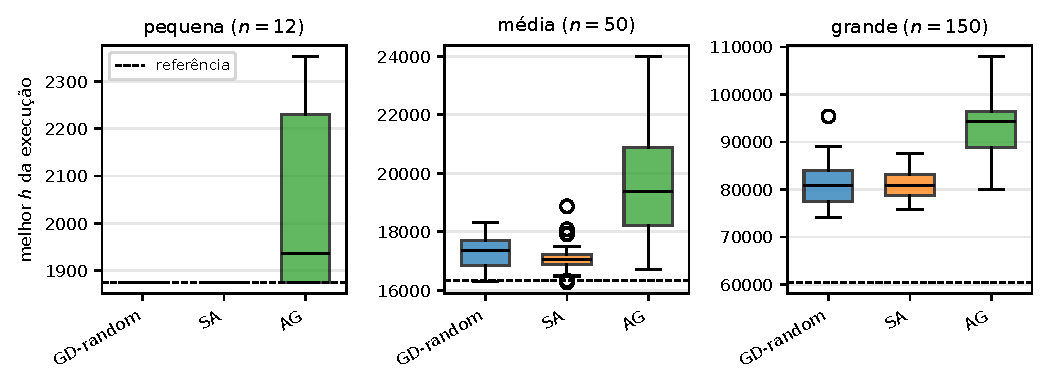
\includegraphics[width=\textwidth]{boxplots}
  \caption{Melhor $h$ por execução. A linha tracejada é o valor de referência da Tabela~\ref{tab:instancias}.}
  \label{fig:boxplots}
\end{figure}

A descida gulosa e o SA não se distinguem estatisticamente em nenhuma instância ($p = 1{,}000$, $0{,}145$ e $0{,}910$).
O SA tem a menor mediana na média e na grande, mas com essa dispersão a diferença não autoriza conclusão.
Os dois vencem o AG nas três instâncias, com $A_{12}$ entre 0,80 e 0,93.
Na grande, onde há só 10 execuções, a vantagem continua significativa ($p$ com Holm de 0,015 e 0,004).
Três execuções na instância média ficaram abaixo da referência publicada: SA com 16\,269, GD-random com 16\,306 e, no experimento extra, o AG memético com 16\,234 (Tabela~\ref{tab:melhores}).
Na grande, a melhor solução que encontramos, 68\,986, ainda está 14\% acima da referência.

\begin{figure}[tbp]
  \centering
  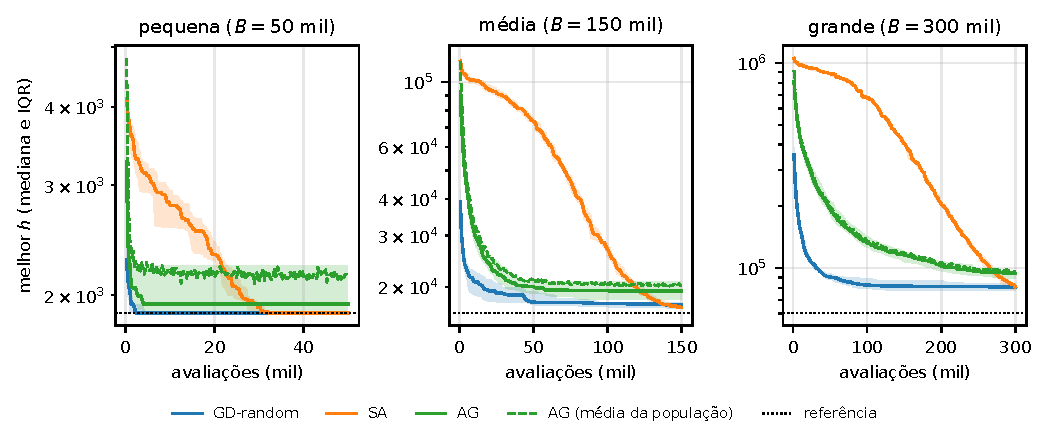
\includegraphics[width=\textwidth]{convergencia}
  \caption{Convergência: mediana (linha) e intervalo interquartil (faixa) do melhor $h$ encontrado até cada avaliação, em escala logarítmica. A linha tracejada verde é a mediana do $h$ médio da população do AG.}
  \label{fig:convergencia}
\end{figure}

As curvas de convergência (Figura~\ref{fig:convergencia}) mostram três dinâmicas diferentes com o mesmo orçamento.
A descida gulosa desce quase toda a distância nas primeiras avaliações e depois avança aos saltos, a cada reinício que encontra um ótimo local melhor.
O SA fica muito acima das outras duas por metade do orçamento, enquanto a temperatura ainda aceita a maior parte das pioras, e só alcança a descida gulosa no fim.
No AG, a curva da média da população passa a acompanhar de perto a do melhor indivíduo depois das primeiras gerações, sinal de que a população ficou homogênea; a distância que sobra, mais visível na pequena, vem dos mutantes criados a cada geração.

\paragraph{Tempo $\times$ avaliações.}
As execuções gastam o mesmo número de avaliações, mas não o mesmo tempo: na grande, 3,8\,s na descida gulosa, 6,0\,s no SA e 8,4\,s no AG, ou cerca de 13, 20 e 28\,µs por avaliação.
O SA também avalia de forma incremental, mas sorteia e calcula uma exponencial a cada passo e reconstrói o prefixo a cada movimento aceito, o que nele acontece com muito mais frequência.
O AG avalia cada filho do zero, porque o filho do OX não compartilha prefixo com uma solução já avaliada, e ainda paga o cruzamento.
Contar avaliações mede o esforço de busca independentemente da implementação e da máquina; com um orçamento de tempo, a vantagem das buscas locais sobre o AG seria ainda maior.
